\documentclass[12pt]{article} 
\usepackage{graphicx}
\def\baselinestretch{2.0}
\setlength{\topmargin}{0pt}
\setlength{\textheight}{570pt}
\setlength{\oddsidemargin}{0pt}
\setlength{\evensidemargin}{60pt}
\setlength{\textwidth}{427pt}
%\setlength{\footheight}{0pt}
\setlength{\footskip}{30pt}
\parindent 15pt
\hyphenpenalty=10000
\tolerance=10000
\pagestyle{empty}

\begin{document}

\centerline{\bf From population genetics to evolutionary genetics: a
view through the trees}
\bigskip

\begin{center}
Joseph Felsenstein\footnote{E-mail address: joe@genetics.washington.edu}\\
Department of Genetics\\
University of Washington\\
Box 357360\\
Seattle, Washington 98195-7360, USA
\end{center}
\newpage


This is a personal and impressionistic account of the situation in
evolutionary genetics and molecular evolution, as it seemed to one
participant in theoretical and methodological developments in those
fields.  It is based in part on a Presidential Address delivered to the
Society for the Study of Evolution at its 1993 annual meeting in
Snowbird, Utah.

\section*{Theory reaches its zenith}

During the years I spent in the Lewontin lab (1964-1967), population genetics was
a quite different field than evolutionary genetics is now.  Theoretical
population genetics had a tradition dating back before Hardy and
Weinberg, and was a reasonably mature field.  We spent our time making various
evolutionary forces collide with each other, as experimental physicists do with
particles.  The intention was to try to discover general laws about which force
would prevail.   There was a great need for total generality, for a simple reason --
there were almost no data to be had, so that we could not constrain
our conclusions to particular parts of the parameter space.  As we could not
know how large selection coefficients were, or what were the patterns of
gene interaction, we needed results that would be general across all of
them.  The theory was
beautiful indeed: the Kolmogorov equations as masterfully employed by Kimura,
and the variance components machinery of Fisher and Wright, burnished to a high
polish by Kempthorne and Cockerham.

Outside of this beautiful but small world was the frightening reality of
interspecies differences, about which we could say almost nothing.  In about
1970, evolutionary biology looked to us as it does in Figure 1.
Our central obsession was finding out what function evolution would try to
maximize.  Population geneticists used to think, following Sewall Wright,
that mean relative fitness, $\bar{w}$, would be maximized by natural
selection.  This is true for one locus, as long as the relative fitnesses
remain constant.  But by 1966 work on multi-locus systems had advanced
from its inception by Kimura (1956) and Lewontin and Kojima (1960).
We now knew (Moran 1966) that $\bar{w}$ could decline as a
result of natural selection and recombination, even decline steadily.
It had already been known to Fisher and Wright that if the fitnesses
changed secularly or as a result of gene frequency dependence, the
result would usually be a failure to maximize mean relative fitness.  But
Moran's result was shocking -- the failure to maximize $\bar{w}$ had invaded
even the case of constant relative fitnesses.

If only we could find out what function other than $\bar{w}$ was
maximized by natural selection in the presence of recombination,
we would have some insight into what compromises
occur between the genetic machinery and natural selection.
We might then also be able to see what selection would to the genetic system
itself, and to 
what extent mean fitness, and hence adaptation, would be expected to be
increased in evolution.

Two technological revolutions came to the field.  One was the
availability of computers.  They were first employed in biology in solving
the selection-migration cline (Fisher 1950; see Wilkes 1975).  In 1954,
the original and eccentric Nils Aall Barricelli was the first to use
them for genetic simulation (Barricelli 1954), partly because he was
one of the first to have access to a computer.  Barricelli's work was not
published until later in English, and so it fell to Fraser (1957a, b) to do the
first widely-noticed genetic simulations.  By the early 1960s genetic
simulation, numerical iteration of deterministic equations, numerical
solution of equilibria in deterministic cases, and numerical evaluation
of equilibrium distributions in stochastic ones, were all standard tools.
They made the investigation of multi-locus natural selection possible.

Of course, in the absence of data to constrain the parameters, we really needed
general theorems, not computer simulations.  The late 1960s and early 1970s
were therefore also the time that mathematical rigor first arrived in
population genetics.  Previous theoretical work had been to an engineering
standard of
rigor rather than a mathematical standard.  Approximations were made, and
small quantities tossed out of the expressions, seemingly arbitrarily.  This
often worked well, but sometimes we divided 0 by 0 and deluded ourselves.
Now, however, we had serious mathematicians
like Samuel Karlin heavily involved in population genetics.  It would surely
be only a matter of time before general results flowed forth, including the
long-sought maximization principle.  The journal {\it Theoretical Population
Biology} was at the cutting edge of this revolution.

But in spite of the best efforts of a lot of fine mathematicians, and
the earnest fumblings of the rest of us, the general results we hoped for did
not turn
out to be accessible.
Most of the
proofs that
emerged were demonstrations that particular proposed generalizations were {\it not}
correct, leaving us all still frustrated.  It is fairly clear that these
failures were not the fault of the researchers; the problems simply
did not have tractable solutions.

There is no theorem that says that mean fitness, or even mean relative
fitness, must be improved when natural selection acts on Mendelian genetic
systems.  Mendelian genetic systems are not optimally designed to be the
ones most friendly to adaptation.  The genetic phenomena, such as
recombination, can make fitness decline.  Nevertheless, it is equally
clear that adaptation does occur a reasonable fraction of the time.  If it
did not, we would not be here to read this volume.  Our genetic system is
not optimal, it is merely good enough.  Its ability to adapt effectively
may not be
perfectly general, but may depend on which part of a parameter space of biological
systems we live in.  If gene interactions were more complex, perhaps we would
rarely be able to adapt.  The average progress in adaptation of Mendelian genetic
systems may be something which we could not know without
knowing more about where we are in the space of potential gene interactions.
Wagner and Altenberg (1996) have raised the issue of the ``evolution of adaptability"
and shown an example of an evolving system tending to move into
regions of parameter space that allow it to successfully adapt.

The area in which theoretical population genetics succeeded best during
this period was in the study of life history evolution.  Following the lead of
W. D. Hamilton
and John Maynard Smith, particular genetic phenomena in life histories
received theoretical treatments that expanded our understanding of
how the life cycles of organisms have come to differ.  While some phenomena,
such as the evolution of recombination, have remained mired in controversy,
others have yielded to theory.  Some of the high points for me have been
Hamilton's (1967) investigations of variations in equilibrium sex ratios,
Maynard Smith's ``cost of meiosis" (1971), Brian Charlesworth
solving the mystery of why Y chromosomes degenerate (1978), and insight from
Marc Feldman's lab into modifier evolution (cf. Altenberg and Feldman 1987).

These undoubted successes have, however, affected only life history traits.
They leave us without any better understanding of the elephant's trunk, or
the Panda's thumb.  Some of the ``monsters" who lurked outside the species
barrier in the 1970s were actually morphological evolutionists, who
roamed the hallways of our departments, desperately seeking someone to help
them analyze their data.   Among ourselves, population geneticists used to
boast about how little help we had given.  ``Fred Bloggs came to see me with
his meaningless snail data.  I threw him out." (laughter)

Under these circumstances, morphologists could be forgiven for concluding that
population genetics theory was useless to them, and for trying to find a
different evolutionary theory that spoke to their concerns.  One of the
attractions of species-selection forms of punctuationism, for example, was that
in one stroke they demoted all within-population genetic phenomena to
the mere generation of variability, with the interesting natural selection
occurring above the species level.  This was a satisfying response to
unhelpful population geneticists.

And yet, population genetics {\it had} already delivered insights into morphological
evolution.  The theory {\it has} succeeded in giving us a quantitative feel for
the relative strength of various evolutionary forces.  We can use it to show
how slow change would be if driven only by mutation, how small
selection coefficients must be to have their effect swamped by random genetic
drift, and how much migration would be needed to overwhelm local adaptation.
All of these might also have been attempted using another theory of
inheritance, such as the blending inheritance
theory of Fleeming Jenkin (1867), but the results would have been very different.
Our current understanding of when migration, mutation, or genetic drift
can be invoked to explain an unusual pattern derives directly from the
mathematical implications of Mendelian inheritance, as assimilated into 
evolutionary theory during the period of the Modern Synthesis.
The fact that we could not be of much practical help to morphological
evolutionists has tended to obscure this fact.


\section*{Enter the data}

What was needed was data, and here a second technological revolution
had a more dramatic effect.  When I was a graduate student,
Lewontin and Hubby (1966) were working on some obscure project involving
electrophoretic gels.  It seemed a bit odd, so we other members of
the Lewontin lab felt fortunate in not being made to work on it.  As soon
as their paper had appeared, it was immediately obvious that the field
was transformed: where there had been little data there was now a lot.
A wave of excitement swept population genetics, and
extravagant promises were made. If we could only compute
the right statistic from them, electrophoretic gene frequencies would solve
the problem of discriminating between neutrality and selection.  But this was
not to be, and as the
years wore by, both lecture audiences and granting agencies became wary of the
claim that we would solve this problem Real Soon Now.  
The reason for the failure was simple -- natural selection, with
millions of generations and vast population sizes, can detect far smaller
selection coefficients than we can hope to in any experiment.  It should
therefore have been anticipated that we were not going to be able to
discriminate between neutrality and weak selection as well as evolution could.

Nevertheless, the revolution wrought by the arrival of molecular biology
has been vast.  It was now relatively easy to generate multiple-locus
gene frequency data within species by electrophoretic techniques.

The need for methods to analyze these data was great, and population
geneticists responded.  One landmark was Ewens's (1972) derivation
of the likelihood for a single locus sample from an infinite-alleles model,
with the surprising conclusion that the number of alleles was the sufficient
statistic for the parameter $\theta = 4N_e\mu$, the scaled product of effective
population size and neutral mutation rate.  As real data are likely to
also contain some deleterious alleles as well, we cannot actually draw from
this the conclusion that gene frequencies do not matter in this estimation.
Watterson (1975) put forward the infinite-sites model and explored the
estimation problems that it raises, suggesting the Number of Segregating
Sites statistic as useful for estimating $\theta$.

Another landmark was Nei's (1972) genetic distance, which became an
important tool near the species level.  Even if we could not resolve the
neutrality-selection controversy, we could use tools based on neutrality
to ask other questions about population structure and history.  In fact, one
might say that the failure to resolve the neutrality-selection controversy
actually strengthened the use of these tools.  For if there was no easy way
to discriminate between the gene frequency patterns expected under neutrality
and under selection, one could simply use the neutrality
theory to generate expectations, secure in the conviction that the presence
of selection would change these patterns very little.

Twenty years on, we can see that these methods of data analysis had a greater
effect than the pure theory done during the same period.  To a considerable extent the change from
``population genetics" to ``evolutionary genetics" has been a change from
a field that was theory-driven to one that is driven by data analysis.

\section*{Into the trees -- the rise of molecular evolution}

While population genetics was turning into evolutionary genetics, other kinds of
molecular
data and other uses of computers were also revolutionizing the analysis of
between-species data.  With molecular sequences available, precisely comparable
data at the
genetic level became available across multiple species.  Previously, there had
been some chromosome banding data, but only in certain groups.  Morphological data
suffered from having an unknown genetic basis, so that it could not give
information at the genetic level.

It took only a few years from the first protein sequences to the first
sequence comparisons between species.  Zuckerkandl and Pauling (1962) were
the pioneers.  They foresaw a ``chemical paleogenetics" in which ancestral
protein sequences could be reconstructed from contemporary comparisons, and
in their work the molecular clock was first postulated.  As the 1960s
progressed, protein sequences for multiple species accumulated.  The publication
of the Atlas of Protein Sequences by the late Margaret Dayhoff (Eck and Dayhoff,
1966) was
important in bringing evolution to the attention of molecular biologists, and
molecular biology to the attention of evolutionists.  Dayhoff took an uncompromisingly
evolutionary approach to the data she compiled; the Atlas was, from the start,
full of phylogenies and discussions of phylogenetic methods.

Suddenly, molecular biology started answering open questions about the
evolutionary history of organisms.  In the hands of Morris Goodman (1963a 1963b)
Vincent Sarich, and Allan Wilson (Sarich and Wilson 1967), humans were relocated within the great apes (rather than being a
sister group to them), and within the African apes, and finally made the
nearest relative of the chimpanzees by Sibley and Ahlquist (1984).  The date
of human-chimp divergence was reduced to 5 million years by Wilson and Sarich (1969).
Similar revolutions affected other groups.  Woese and Fox (1977) separated the
Archebacteria from the Eubacteria, alough the Archaebacteria subsequently proved to be
a bit less archaic than their name implied.  In many other groups, molecular
evidence had a less disruptive effect, confirming the historical reconstructions
of morphologists more than it contradicted them.  But especially where morphology
faltered, molecular evolution was magically effective.

\section*{Numerical methods for molecular evolution}

As the number of species in molecular data sets increased beyond a few, it became
necessary to come up with a numerical methology for reconstructing phylogenies.
This literature had started with Edwards and Cavalli-Sforza's paper of 1964, which is
one of the true landmarks in the phylogenetic literature.  Sadly, it is very little
known among people making phylogenies, because of the misapprehension that this
literature sprang from the work of Willi Hennig (1950, 1966).  The availability of
computers in the 1960s led to the development of methods for inferring
phylogenies. The parsimony and likelihood methods were introduced by Edwards and
Cavalli-Sforza, for blood group polymorphism gene frequencies.  Camin and Sokal (1965)
described the first discrete-characters parsimony method, and Cavalli-Sforza and
Edwards  (1967) one of the first distance-matrix methods.  Molecular evolutionists were involved in
this process very early: Eck and Dayhoff (1966) carried out the first molecular
parsimony analysis, and Walter Fitch (Fitch and Margoliash 1967) used cytochrome sequences to pioneer distance
matrix methods.  Sanger had produced the first protein sequence in
almost the same year that computers became widely available to scientists; ten years
later, all of the major methods of analysis of molecular sequence data had been
introduced, and most had already been applied to molecular data.

At first, these methods did not seem to be making any assumptions about
evolution.  But as distance matrix methods, and later likelihood methods,
became more popular, it was apparent that they necessarily involved models
of evolution.  This point has not been easily appreciated by systematists --
it has taken outsiders to bring models to their attention.  It is noticeable
that, of the originators of the major methods of inferring phylogenies, only
a few were trained as systematists.
The others were population geneticists
(Cavalli-Sforza and Edwards), biochemists (Walter Fitch and Margaret
Dayhoff), medical microbiologists (Peter Sneath), or statisticians (Jerzy
Neyman).  The mathematical perspective did come easily to systematists.

\section*{Unilluminating models}

The simplest models in molecular evolution (e.g, Jukes and
Cantor 1969) were models of ``random hits", in which each site was equally
likely to change, with alternative nucleotides equiprobable when it did change.
These models were based on the observation of an approximate molecular
clock, but without any specification of what evolutionary forces were
creating these changes.

Lewontin and Hubby (1966) had already suggested neutral mutation as a
possible mechanism for electrophoretic polymorphism.  It was Kimura (1968;
Kimura and Ohta 1971) who first integrated within- and between-species
molecular observations by suggesting that both electrophoretic polymorphism
and sequence evolution were the consequence of the same process, neutral
mutation.  This had the effect on evolutionary genetics of bringing more
data to bear, but an even greater effect on molecular evolution.  It supplied
it with a theory, ready-made.

It was immediately apparent that natural selection was acting as well.
Some proteins were evolving rapidly (fibrinopeptides, for example) and
others slowly (histones).  These differences could easily be accomodated
in the neutral mutation theory, which did not postulate that all mutations
were neutral, only that all that caused polymorphism were.  There could
be a fraction of all mutants that did not cause polymorphism
or sequence change because they were deleterious.  It could vary from
site to site and from locus to locus.  It was to be expected that
critically important regions of sequence would have most mutants be
deleterious, and that these would be eliminated by ``purifying" selection.
Models of molecular evolution have undergone modification in recent
years to take these heterogeneities of rate of evolution into account.

Most evolutionary geneticists and molecular evolutionists have agreed that
most noticeable heterogeneities of rate of evolution were caused by the
presence of this purifying selection.   Both committed neutralists and
zealous selectionists have been in agreement on this.  Where they would disagree
was whether the polymorphisms that were seen, and the sequence changes that
were seen, resulted from natural selection or genetic drift.  So far, there
has been little progress in telling these forces apart, either from
within- or between-species data.  This has been frustrating, but, as we
have noted, it has had the
happy effect that data could be analyzed using modified neutral mutation models,
without much threat from the inadequacy of the model.

The result has been that the models used in molecular evolution are
particularly simple, but in some respects disappointing.  They are primarily
models specifying  what does {\it not} happen.  Since we do not know
whether the changes that do happen are the result of positive natural
selection or neutral mutation, there is no way to predict how much natural
selection is expected to improve molecular function.   I often find that when
people outside the field ask what theory predicts about molecular evolution,
they are disappointed to find that its predictions are so negative.

\section*{Sequence samples from populations}

While molecular evolution was maturing as a field, the same molecular
technology was slowly invading evolutionary genetics.  The invasion has been
slow because so much evolutionary genetics was supported by the aptly-named
NSF\footnote{In the USA, NSF means National Science Foundation, and is also
 the abbreviation on your bank statement when you have Not Sufficient Funds}.  It is still much cheaper to do electrophoretic surveys at many
loci than to get one population sample of molecular sequences.  It is
noticeable how long it has taken, since Kreitman's pioneering studies (1983),
for population samples of nuclear molecular sequences to become common.

A major exception must be made for one tiny piece of eukaryotic DNA.
Mitochondrial population samples have been widely used.
They got much attention with the famous ``mitochondrial Eve" study of
Cann, Stoneking and Wilson (1987).   At first, mitochondria were used because their DNA was
easy to extract.  That ceased to be an advantage with the development of
PCR, but other advantages (maternal inheritance, haploidy, and rapid rate of
evolution) have been cited as additional reasons to concentrate on the mitochondrial
genome.

Initially, few of the researchers using mitochondrial data related their
trees to population processes.  The presence of an ``Eve" seemed to be an
unusual consequence of maternal inheritance.  But every nucleotide
in the genome should in principle have its own ``Eve" or ``Adam", as a
result of the coalescent process at that locus.  How far along the genome
one can go and still find that same coalescent tree, so that
every gene copy comes from that same ancestor, depends on the rate of recombination and
the effective population size.   The techniques of molecular evolution
have invaded evolutionary genetics as people began to infer these ``gene
trees".  At the same time evolutionary genetic theory turned out to
provide the theoretical framework for analyzing these gene trees.   The
basic theoretical work was done by J.F.C. Kingman (1982a 1982b).  His work
generalized Sewall Wright's result (1930) for two copies.  Wright pointed
out that two copies of a gene in a closed randomly-mating population would have
a common ancestor an average of $2N_e$ generations ago, with the
distribution being approximately exponential.  Kingman's ``$n$-coalescent"
process (Figure 2) is the generalization of this to $n$ copies.  The time during which all
$n$ copies have had distinct ancestral lineages is exponentially
distributed, with mean $4N_e/n(n-1)$ generations.  Before that, there were
$n-1$ copies, to which the same rule applies, and so on.

Kingman's work is mathematically elegant, but easily applied in practice.  We
do not need to use Kingman's technical machinery to understand and use the
distribution of trees that his work predicts.  The name ``coalescent" has come
to be applied to any gene tree.  Kingman's prediction allows us to make a
statistical analysis of sequence samples from populations.  In principle, when
developed enough, this will allow a statistical analysis of the evidence
which discriminates between the ``Out of Africa" scenario for human
evolution with the ``Multiregional Hypothesis".  At the moment, there is not
a truly statistical methodology for analyzing the data in this controversy.

The key to analyzing population samples of sequences is not to focus too
obsessively on finding the true gene tree.  One will usually have too few
varying sites in the molecule to make an accurate estimate of the gene tree.
It therefore becomes essential to take into account the noise in our
estimate of the gene tree.   There are two main sources of statistical error
in these inferences.  One is the randomness of the coalescent tree itself,
which is drawn from Kingman's distribution.  The other is the error in our
estimate of the coalescent tree, which depends on the randomness of the
mutational processes at molecular sites.

The fundamental equation for likelihood inference in coalescent trees is
(Felsenstein 1988)
\begin{equation}
L = \sum\limits_{G} {\rm Prob\;}(G|\alpha) {\rm Prob\;}(D|G, \mu)
\end{equation}
where $L$ is the likelihood (the probability of the data given the
parameters), $\alpha$ is the collection of parameters for the population
processes (effective population sizes, migration rates, etc.), and $\mu$ is
the neutral mutation rate per site.  The summation over $G$ sums over all
possible coalescent trees that could connect the observed sequences,
counting not only tree topologies but also branch lengths.
Interestingly, the first term inside the summation is the Kingman prior
(or its analogue in the particular case); the second is the standard
likelihood used when phylogenies are being evaluated.

Although these two quantities are easily computed, the sum looks like an
impossible one to compute.  There are vast numbers of forms of the
coalescent tree, and each has an infinite number of possible branch
lengths. For example, with only 10 sequences, to compute (1) we need to compute 
$2.571 \times 10^9$ 9-dimensional integrals!  However, two groups have
developed methods that use random sampling to take a Monte Carlo integration
approach to this sum.  Griffiths and Tavar\'e (Griffiths 1989; Griffiths and Tavar\'e 1994a 1994b)
have taken in place of $G$ the set of all mutational and coalescent sequences
of events, without times of the events.  Equation (1) then can be
written in a recursive form.  They compute the resulting sum by sampling
paths down through the recursion.  This can be extremely fast for sequences
that obey Watterson's infinite sites model, where no mutation ever recurs.
It is less clear how rapidly it can be computed in a finite-sites model,
such as the ones in standard use in studies of molecular evolution.

Our own lab (Kuhner, Yamato and Felsenstein 1995) has used a Metropolis-Hastings
sampler to wander through the space of all possible coalescent trees (Figure 3).  We
do this by starting with a reasonable tree, and gradually modifying it.
This is an example of a Markov Chain Monte Carlo method.  Such methods are
gaining wide acceptance for solving complex statistical problems.
The Metropolis-Hastings sampler works by acceptance or rejection of the
resulting tree,
depending on the value for it of the quantity being summed in equation (1).
After a large sample of possible trees has been built up, an estimate
of the likelihood surface can be made.
Mary Kuhner and Jon Yamato's COALESCE program, available in our LAMARC
package of coalescent likelihood programs\footnote{Available on World Wide Web at http://evolution.genetics.washington.edu/lamarc.html}, seems to compute and maximize
$L$ effectively on workstations and fast microcomputers with large enough
memory.

In effect, the mathematics of likelihoods on phylogenies, and that of
coalescent priors, has come together to provide a set of tools for
likelihood analysis of population samples of sequences.  I suspect that
these will become the standard methods for analyzing these data.

The Metropolis-Hastings sampler averages over our uncertainty about the
coalescent tree, taking our knowledge of that tree into account properly.
One might imagine that this could be made unnecessary.  Suppose that there
was little uncertainty about the coalescent tree.  For example, if we
sequenced entire mitochondria, we could be very sure of its tree topology
and fairly sure of its branch lengths.  In such a case, that
would eliminate the need for the Markov Chain Monte Carlo sampling.
Yet it would not solve the problem.  Looking at a large number of sites
does eliminate the uncertainty that comes from the mutational variability.
But it looks at only one coalescent tree, since the whole mitochondrion
shares one coalescent.  In addition, there is the risk that ``hitchhiking"
natural selection could affect that coalescent, biasing our estimate of
the effective population size.

To eliminate the noise due to the variability of the coalescent itself, we
must look at
many regions of the genome, each of which would have its own coalescent.
That implies that we need population studies of nuclear DNA.  And that
raises the issue of recombination.   It is not hard to generalize
Kingman's formulas to allow for recombination (cf. Hudson and Kaplan 1985).
In the presence of recombination, the coalescent tree becomes a collection
of trees (see Hudson 1990), or a network with loops in it.
However, both Griffiths and Tavar\'e and my own lab have developed
random-sampling methods for trees with recombination.  When these methods
are available, they will make it possible to analyze population samples
of nuclear DNA.   That will in turn allow evolutionary geneticists to
subdue the variability of the coalescent tree itself, not just the
uncertainty of our estimate of it.

\section*{Enter genomics}

These same molecular and computer technologies have brought modern genomics
into existence.  As it is a high-budget technology, it has been even slower to
show up in evolutionary biology, but its presence is now noticeable.  Although
many of the current genomics projects in evolutionary biology are for organisms
that have economic importance, it is becoming possible for evolutionary
biologists to search for major genes affecting traits that they study.

One does not need to be very daring to predict that this trend will continue.  Of course,
if traits are controlled by large numbers of loci of small
effect, it will fail to explain them.  To the extent that it succeeds,
the classical variance components techniques will recede from view.   In some
cases the identification of QTLs can resolve old dilemmas.  For example,
suppose that we see a trait differing between two populations.  Has this
difference arisen because of genetic drift, or selection?  And if selection,
was it acting on this trait or on some correlated trait?

If genetic drift acted, we would expect all the loci involved to have
differentiated in gene frequency to approximately equal extents, though in
varying directions.   If
natural selection acted, we would expect the loci of largest effect to show
proportionately more differentiation than those of smaller effect, but
all loci to show differentiation in similar directions.  If natural selection
acted on a correlated trait, we would expect differentiation only in those
loci that affected the correlated trait.

Figures 4 and 5 show the two natural selection cases, in an imaginary
example.  The first one is the result of natural selection on that character,
the second one the result of natural selection on another character, which is
only affected by the loci that are shown with asterisks.  Of course, in
reality the analysis is more complicated than this: there is expected to be
a certain amount of heterogeneity in all these patterns as a result of
genetic drift, and we have to be able to do the appropriate statistical
analysis given that.  But the point is that, without the genomics, we
could not hope to untangle whether the trait in question was the actual
target of natural selection.  With the genomics, it is at least possible to
ask the question.  Other confounded evolutionary forces may be separated for
the first time as well.

There has also been an explosive growth of comparative genomics.  The
existence of genetic maps for multiple species gives us data to discuss
rates and processes of genome rearrangement.  Sankoff and Goldstein (1989) have begun
the process of developing probabilistic models of genome rearrangement.  We
will surely see many more uses of these in evolutionary biology.

\section*{Enter morphometrics?}

Computer technology has led to the development of methods of image
capture and analysis, and those to the development of morphometrics.
Under the leadership of Fred Bookstein and Jim Rohlf, methods are being
developed for analysis of outlines and landmarks, and even both at the same
time.  At the moment, this activity has had little impact on evolutionary
biology, but that will surely change.  When genomics can be done on
quantitative characters affecting shape, morphometrics will be needed to
discover which aspects of shape each locus is affecting.  In between-species
comparisons, there would seem to be much room for use of morphometrics.

At the moment, morphometrics suffers from its methods being purely geometric.
Developmental biology has had no impact on morphometrics, as developmentalists
are unable to provide parameterized models of the development of the
characters.  Thus one has to choose as the basic variables of interest ones
which may not correspond to the developmental parameters.  In fact, the
information may flow in the other direction.  Morphometric studies of
within-population variation may suggest which aspects of form are varying
indpendently, and which in a correlated direction.  The difficulty with this
program of study is that both mutation and natural selection will affect
which aspects of form vary in a correlated fashion.  This is simply a reworking
of the old controversy between quantitative geneticists and morphologists
over whether constraints are important in evolution.  With genomics
available, there could be some resolution in particular cases.

\section*{Really big trees}

As phylogenies grow in size, further questions open up.  It will become
possible to statistically assess the role of species selection, for example.
Kirkpatrick and Slatkin (1993) have studied statistics for testing
imbalance in phylogenies.  With such statistics, we could see whether there
was significant evidence that a trait had been affected by species
selection.  If those clades that had higher values of the trait also seemed to
be more speciose, this would be evidence for a role of species selection.
We need to have large phylogenies to even attempt this, so it will not be
happening very soon.  It is possible to take a large phylogeny and search
for that linear (or even nonlinear) combination of characters that shows the
greatest correlation with clade size.

If the data of paleontologists could be recast from survival of taxa to
phylogenies that have quantitative characters on them, many questions about
long term trends in evolution, as well as natural selection above the species
level could be addressed.

Evolutionary biology in the 1990s therefore no longer looks like Figure 1.
The species boundary holds few terrors, and within- and between-species
variation can be studied together (Figure 6).


\section*{Continuing frustrations}

In some areas there does not seem to be the progress that we need.  We need
a developmental biology that finds repeatable patterns, and hence canonical
models, among different developmental processes.  But if development, like
life, ``is just one damned thing after another", then general models of
developmental biology will lend little aid to evolutionary biology.  The
same is true of ecology.  Although it is intrinsically a more important
field than evolution, it is noticeable how little successful theory is
available in ecology.  When I was a graduate student, Robert MacArthur's
work seemed to promise that strong ecological models of the Lotka-Volterra
type would be available.  Those models have succumbed to skepticism,
leaving ecology as one of the few biological fields where postmodernism
has made any inroads\footnote{(joke)}.   We are thus unable to
connect our molecular and morphological inferences with strong and stable
developmental or ecological models.

\section*{Emergent properties?}

In the absence of developmental generalities, one interesting approach has been
to seek generalizations that will apply to large classes of developmental
systems.  Stuart Kauffman has form many years been investigating
the evolutionary implications of randomly connected developmental systems
(summarized in Kauffman 1995).  His NK model has two parameters that
allow the complexity of the gene interaction to be varied.  There is
certainly reason to believe that it does not resemble the structure of
real biological systems, but it is a daring attempt to pose the question
more generally.  It is just beginning to get the attention it deserves from
evolutionary theorists.  Years ago, I made (Felsenstein 1978) another
long-term evolutionary model, an attempt
to model the energetics of an evolving ecosystem.  The crucial result, that
the total energy content of the evolving ecosystem would rise linearly
with time, depended on one tail of the initial distribution of the efficiency
of energy retention being a power curve.  Even if this is realistic, which
is open to considerable doubt, there is no way at present to connect it to
a mechanistic model of the organism.  It would be wonderful if models like 
these, that attempt to model the long-term course of evolution,
could be interconnected and placed in a more general context.  If such
efforts fail, we can always fall back on the hope that there are some
empirically valid generalizations that can be made about developmental and
ecological interactions.

\section*{A new synthesis?}

After the success of the Neodarwinian Synthesis in the period 1920-1950,
connecting evolution and genetics in powerful ways, it is tempting to try to
discern another new synthesis.  There is certainly a synthesis of
molecular biology and evolutionary biology going on.  Nor does the
influence run in only one direction, as molecular biologists have
discovered that population variation can help them find out which regions
of a genome are under constraint against change.  But at another level
there is no new synthesis.  In the original synthesis, the formal structure
of genetic systems came to evolutionary biology, and resulted in the
mathematical theory of population genetics, easily the most elaborate
body of theory in biology.   In the present syntheses, no new theory has
yet arisen.  The forces invoked are those that we already knew about
within populations.  We have a post-neo-Darwinian synthesis without a
post-neo-Darwinism or, at least, without a new theory.  We have many
new statistical and computational methods, but all use the pre-existing
theory as their base.

Making such a theory is a major challenge.  It probably involves asking
a new set of questions, and seeking generalizations at a higher level.  It
may need to wait for developmental biology and ecology to come up with
some new generalizations.  Or it may simply need a new generation of
evolutionary biologists who can ask a new set of questions. 

\section*{Acknowledgments}

This paper is a revised version of a Presidential Address delivered at the
annual meeting of the Society for the Study of Evolution
in June, 1993 in Snowbird, Utah.  I am grateful to David Fogel for
pointing out the priority of the late Nils Aall Barricelli in the invention
of genetic simulation.  Some of the research reported was supported by grant numbers
2 R55 GM41716-04 and 1 R01 GM51929-01 from the National Institutes of Health, and
grant numbers DEB-9207558, and BIR-9527687 from the National Science Foundation.


\section*{References}
{\parindent=-15pt

{~~}

Altenberg, L., and Feldman, M. W. (1987). Selection, generalized transmission and the
evolution of modifier genes. I. The reduction principle.  {\it Genetics}
 117:559-72.

N. A. Barricelli. (1954).  Esempi Numerici di Processi di Evoluzione.  {\it Methodos}
pp. 45-68.

Camin, J. H., and Sokal, R. R.  (1965).  A method for deducing branching sequences
in phylogeny.  {\it Evolution}  19:311-326.

Cann, R. L., Stoneking, M., and Wilson, A. C.  (1987).  Mitochondrial DNA and
human evolution.  {\it Nature}  325:31-36.

Cavalli-Sforza, L. L., and Edwards, A. W. F.  (1967).  Phylogenetic analysis:
models and estimation procedures. {\it Evolution}  32:550-570 (also published in
{\it American Journal of Human Genetics}  19:233-257.

Charlesworth, B.  (1978).  Model for the evolution of Y chromosomes and dosage
compensation. {\it Proceedings of the National Academy of Sciences, USA}
 75:5618-5622.

Eck, R. V., and Dayhoff, M. O.  (1966). {\it Atlas of Protein Sequence and Structure 1966.}
Silver Spring, Maryland: National Biomedical Research Foundation.

Edwards, A. W. F., and Cavalli-Sforza, L. L.  (1964).  Reconstruction of
evolutionary trees.  In {\it Phenetic and phylogenetic classification,}
ed. V. H. Heywood and J. McNeill, pp. 67-76.  London: Systematics Association Publication No. 6.

Ewens, W. J.  (1972).
The sampling theory of selectively neutral alleles
{\it Theoretical Population Biology}  3:87-112,240,376.

Felsenstein, J. (1978).  Macroevolution in a model ecosystem.
{\it American Naturalist}  112:177-195.

Felsenstein, J. (1988). Phylogenies from molecular sequences: inference and
reliability.  {\it Annual Review of Genetics}  22:521-565.

Fisher, R. A.  (1950).
Gene frequencies in a cline determined by selection and diffusion
{\it Biometrics}  6:353-361.

Fitch, W. M., and Margoliash, E. (1967). Construction of phylogenetic trees.
{\it Science}  155:279-284.

Fraser, A. S. (1957a).
Simulation of genetic systems by automatic digital computers. I. Introduction
{\it Australian Journal of Biological Sciences}  10:484-491.

Fraser, A. S. (1957b).
The simulation of genetic systems by automatic digital computers. II. The effect
s of linkage on the rates of advance under selection
{\it Australian Journal of Biological Sciences}  10:492-499.

Goodman, M.  (1963a).  Man's place in the phylogeny of the primates as reflected
in serum proteins.  In {\it Classification and Human Evolution,}
ed. S. L. Washburn, pp. 204-234.  Chicago: Aldine.

Goodman, M. (1963b).  Serological analysis of the systematics of recent
hominoids.  {\it Human Biology}  35:377-436.

Griffiths, R. C.  (1989).  Genealogical tree probabilities in the
infinitely-many-site model.  {\it Journal of Mathematical Biology} {\bf 27:}
667-680.

Griffiths, R. C., and Tavar\'e, S.  (1994a).
Sampling theory for neutral alleles in a varying environment.
{\it Philosophical Transactions of the Royal Socety of London, Series B (Biological Sciences)}  344:403-10.

Griffiths, R. C., and Tavar\'e, S.  (1994b).  Ancestral inference in population
genetics.  {\it Statistical Science}  9:307-319.

Hamilton, W. D. (1967).  Extraordinary sex ratios. {\it Science} {\bf 156:}
477-488.

Hennig, W. (1950).  {\it Grundz\"uge einer Theorie der Phylogenetischen Systematik.}
Berlin: Deutscher Zentralverlag.

Hennig, W.  (1966). {\it Phylogenetic Systematics.}
(translated by D. D. Davis and R. Zangerl). Urbana: University of Illinois Press
.

Hudson, R. R., and Kaplan, N. L. (1985). Statistical properties of the number
of recombination events in the history of a sample of DNA sequences.
{\it Genetics}  111:147-164.

Hudson, R. R.  (1990).  Gene genealogies and the coalescent process.
{\it Oxford Surveys in Evolutionary Biology}  7:1-44.

Jenkin, F.  1867.
Origin of Species. {\it North British Review}  46:277-318.

Jukes, T. H., and  Cantor, C. (1969).  Evolution of protein molecules. 
In {\it Mammalian Protein Metabolism}, ed. M. N. Munro, pp. 21-132. New York: Academic
Press.

Kauffman, S. A.  (1993).  {\it The Origins of Order.}  New York and London: Oxford University Press.

Kimura, M.  (1956).
A model of a genetic system which leads to closer linkage by natural selection
{\it Evolution}  10:278-287.

Kimura, M. (1968).  Evolutionary rate at the molecular level.
{\it Nature}  217:624-626.

Kimura, M., and Ohta, T.  (1971).  Protein polymorphism as a phase of molecular evolution.
{\it Nature}  229:467-469.

Kingman, J. F. C. (1982a).  The coalescent.  {\it Stochastic Processes and Their
Applications}   13:235-248.

Kingman, J. F. C. (1982b).  On the genealogy of large populations.  {\it
Journal of Applied Probability}  {\bf 19A:} 27-43.

Kirkpatrick, M., and Slatkin, M.  (1993).  Searching for evolutionary patterns
in the shape of a phylogenetic tree.  {\it Evolution}  47:1171-1181.

Kreitman, M.  (1983).  Nucleotide polymorphism at the alcohol dehydrogenase
locus of
{\it Drosophila melanogaster}.  {\it Nature}  304:412-417.

Kuhner, M. K., Yamato, J., and Felsenstein, J. (1995).
Estimating effective population size and mutation rate from sequence data
using Metropolis-Hastings sampling. {\it Genetics}  140:1421-1430.

Lewontin, R. C., and Kojima, K. (1960).
The evolutionary dynamics of complex polymorphisms {\it Evolution} {\bf 14:}
458-472.

Lewontin, R. C., and Hubby, J. L. (1966).
A molecular approach to the study of genic heterozygosity in natural populations
. II. Amount of variation and degree of heterozygosity in natural populations of
 {\it Drosophila pseudoobscura}.
{\it Genetics}  54:595-609.

Maynard Smith, J.  (1971).  The origin and maintenance of sex.
pp. 163-171 in {\it Group Selection,} ed. G. C. Williams. Chicago: Aldine-Atherton.

Moran, P. A. P.  (1966).  On the nonexistence of adaptive topographies.
{\it Annals of Human Genetics}  27:383-393.

Nei, M. (1972).  Genetic distance between populations
{\it American Naturalist}  106:283-292.

Sankoff, D., and Goldstein, M.  (1989).  Probabilistic models of genome
shuffling.  {\it Bulletin of Mathematical Biology}  51:117-124.

Sarich, V. M., and Wilson, A. C.  (1967).  Immunological time scale for
hominid evolution. {\it Science}  158:1200-1203.

Sibley C. G., and Ahlquist, J. E. (1984).  The phylogeny of the hominoid primates, as
indicated by DNA-DNA hybridization. {\it Journal of Molecular Evolution}  20:2-15.

Wagner, G. P., and Altenberg, L.  (1996).  Perspective: complex adaptations and
the evolution of adaptability.  {\it Evolution}  50:967-976.

Watterson, G. A.  (1975).  On the number of segregating sites in genetical
models without recombination.  {\it Theoretical Population Biology}  7:256-276.

Wilkes, M. V.  (1975).  How Babbage's dream came true.  {\it Nature}   257:541-544.

Wilson, A. C., and Sarich, V. M.  (1969).  A molecular time scale for human
evolution.  {\it Proceedings of the National Academy of Sciiences, USA.}  63:1088-1093.

Woese, C. R., and Fox, G. E.  (1977).
Phylogenetic structure of the prokaryotic domain: the primary kingdoms.
{\it Proceedings of the National Academy of Sciences, USA}  74:5088-5090.

Wright, S. (1930).  Evolution in Mendelian populations.
{\it Genetics}  16:97-159.

Zuckerkandl, E. and Pauling, L.  (1962).  Molecular disease, evolution, and
genetic heterogeneity.  In {\it Horizons in Biochemistry,}
ed. M. Marsha and B. Pullman, pp. 189-225. New York: Academic Press.

\newpage

\section*{Figure Captions}
\bigskip

{~~}

Fig. 1 -- A cartoon of the state of population genetics in 1970
\bigskip

Fig. 2 -- Kingman's coalescent process.
\bigskip

Fig. 3 -- The Metropolis-Hastings sampler.
\bigskip

Fig. 4 -- A genetic map showing differentiation of gene frequencies of loci
drift.
\bigskip

Fig. 5 -- A genetic map showing differentiation of gene frequencies of loci
affecting a quantitative character, when population divergence is by
natural selection on a correlated character.
\bigskip

Fig. 6 -- A cartoon of the state of evolutionary biology in the 1990s.
\bigskip

}
\newpage

\begin{figure}[tbhp]
\begin{center}
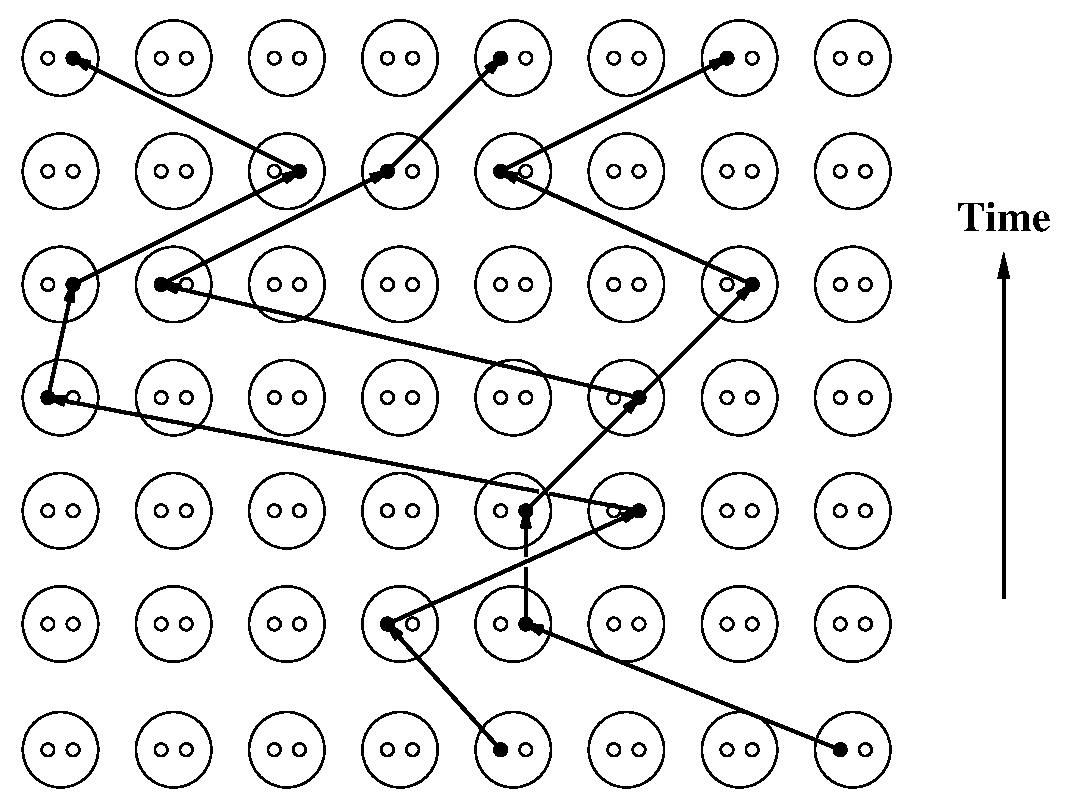
\includegraphics[width=6in]{fig1.idraw}
{\caption ~~}
\end{center}
\end{figure}
\begin{figure}[tbhp]
\begin{center}
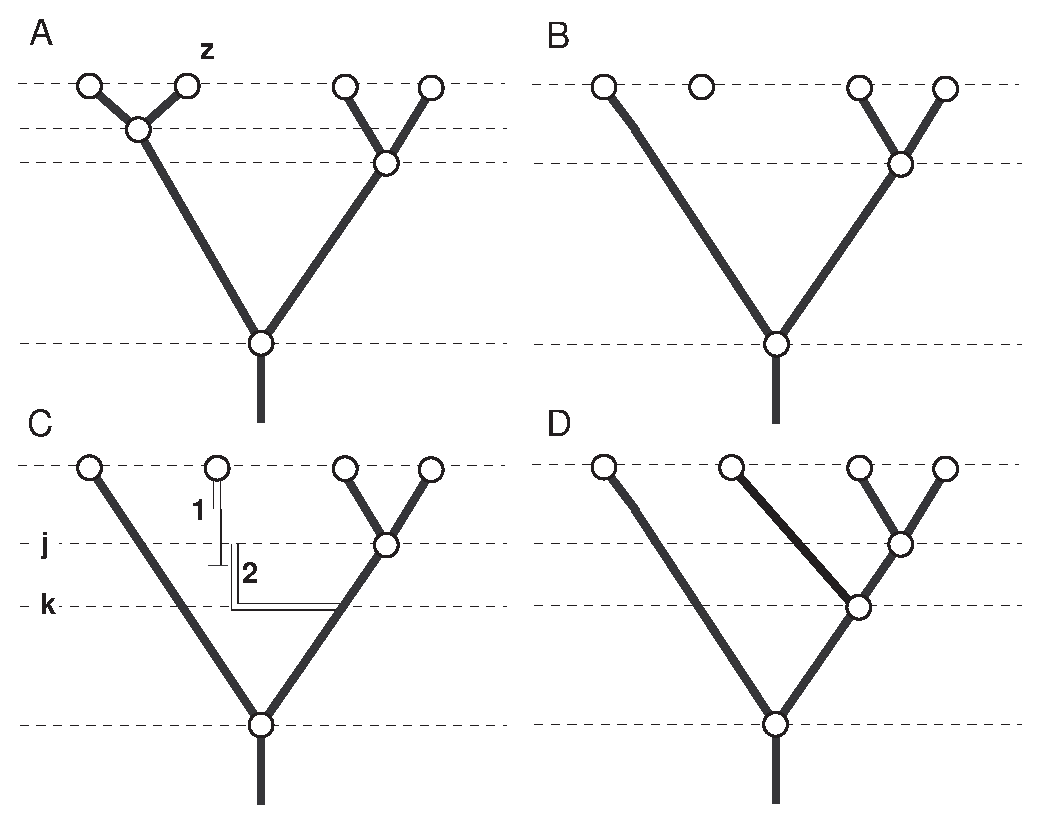
\includegraphics[width=6in]{fig2.idraw}
{\caption ~~}
\end{center}
\end{figure}
\begin{figure}[tbhp]
\begin{center}
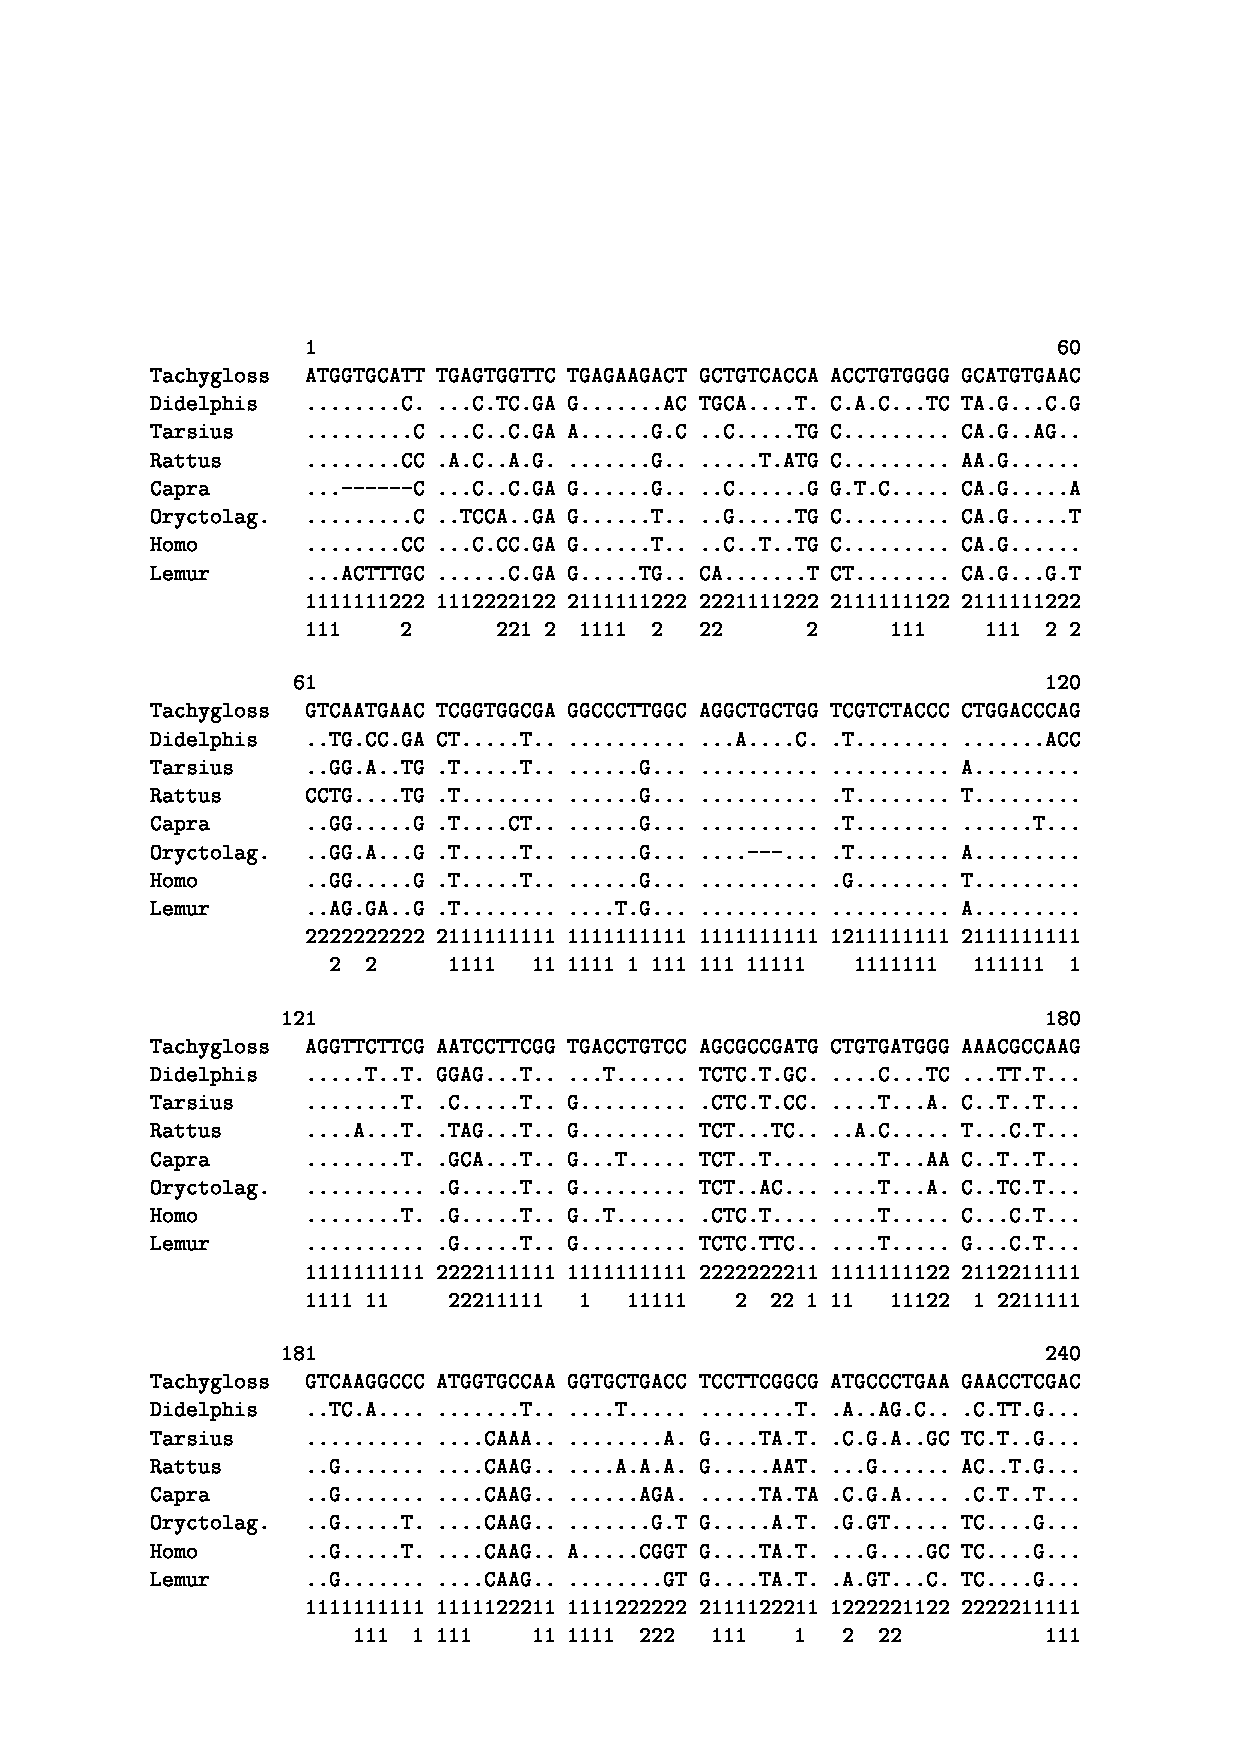
\includegraphics[width=6in]{fig3.idraw}
{\caption ~~}
\end{center}
\end{figure}
\begin{figure}[tbhp]
\begin{center}
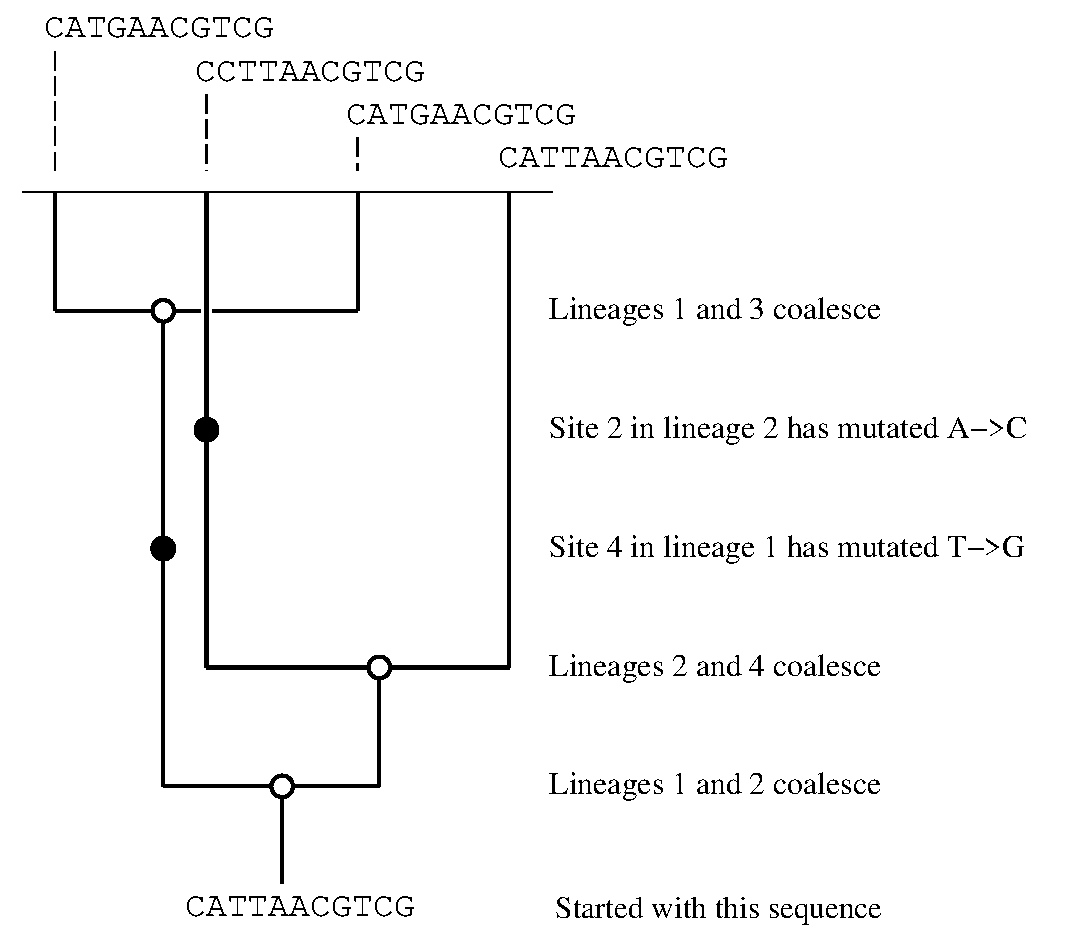
\includegraphics[width=6in]{fig4.idraw}
{\caption ~~}
\end{center}
\end{figure}
\begin{figure}[tbhp]
\begin{center}
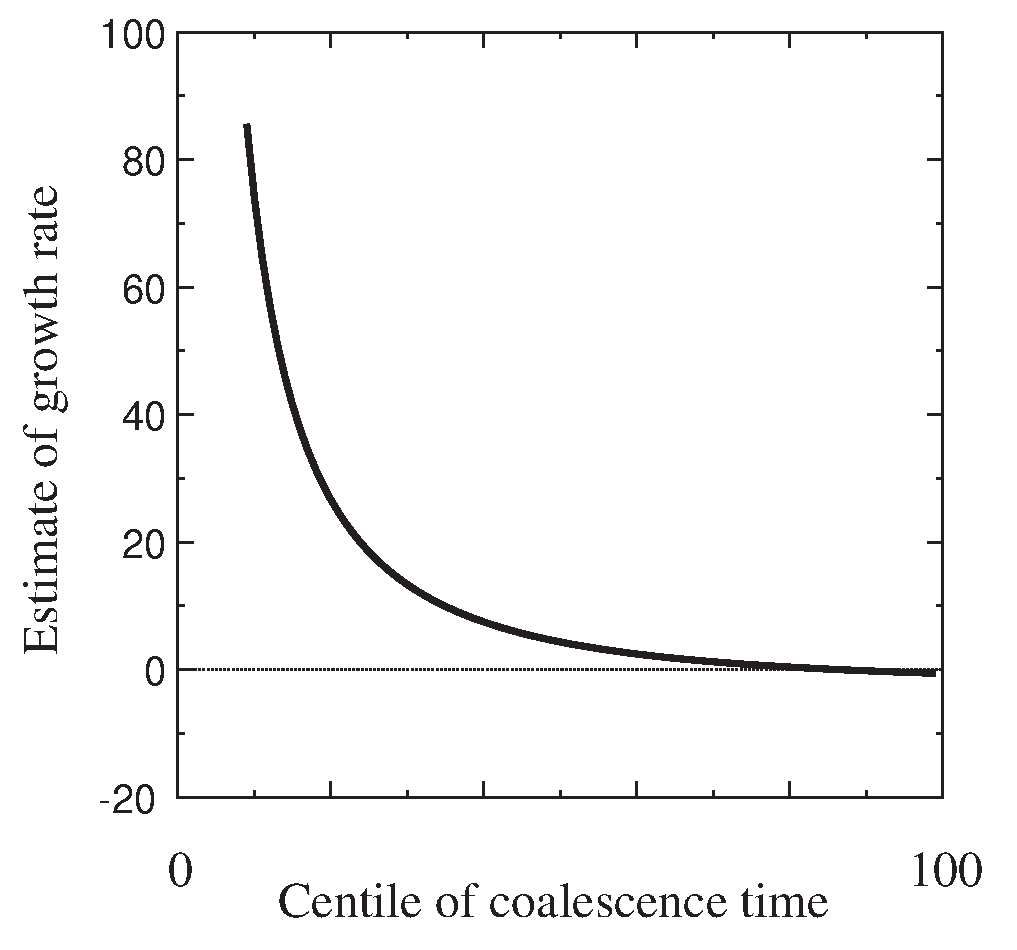
\includegraphics[width=6in]{fig5.idraw}
{\caption ~~}
\end{center}
\end{figure}
\begin{figure}[tbhp]
\begin{center}
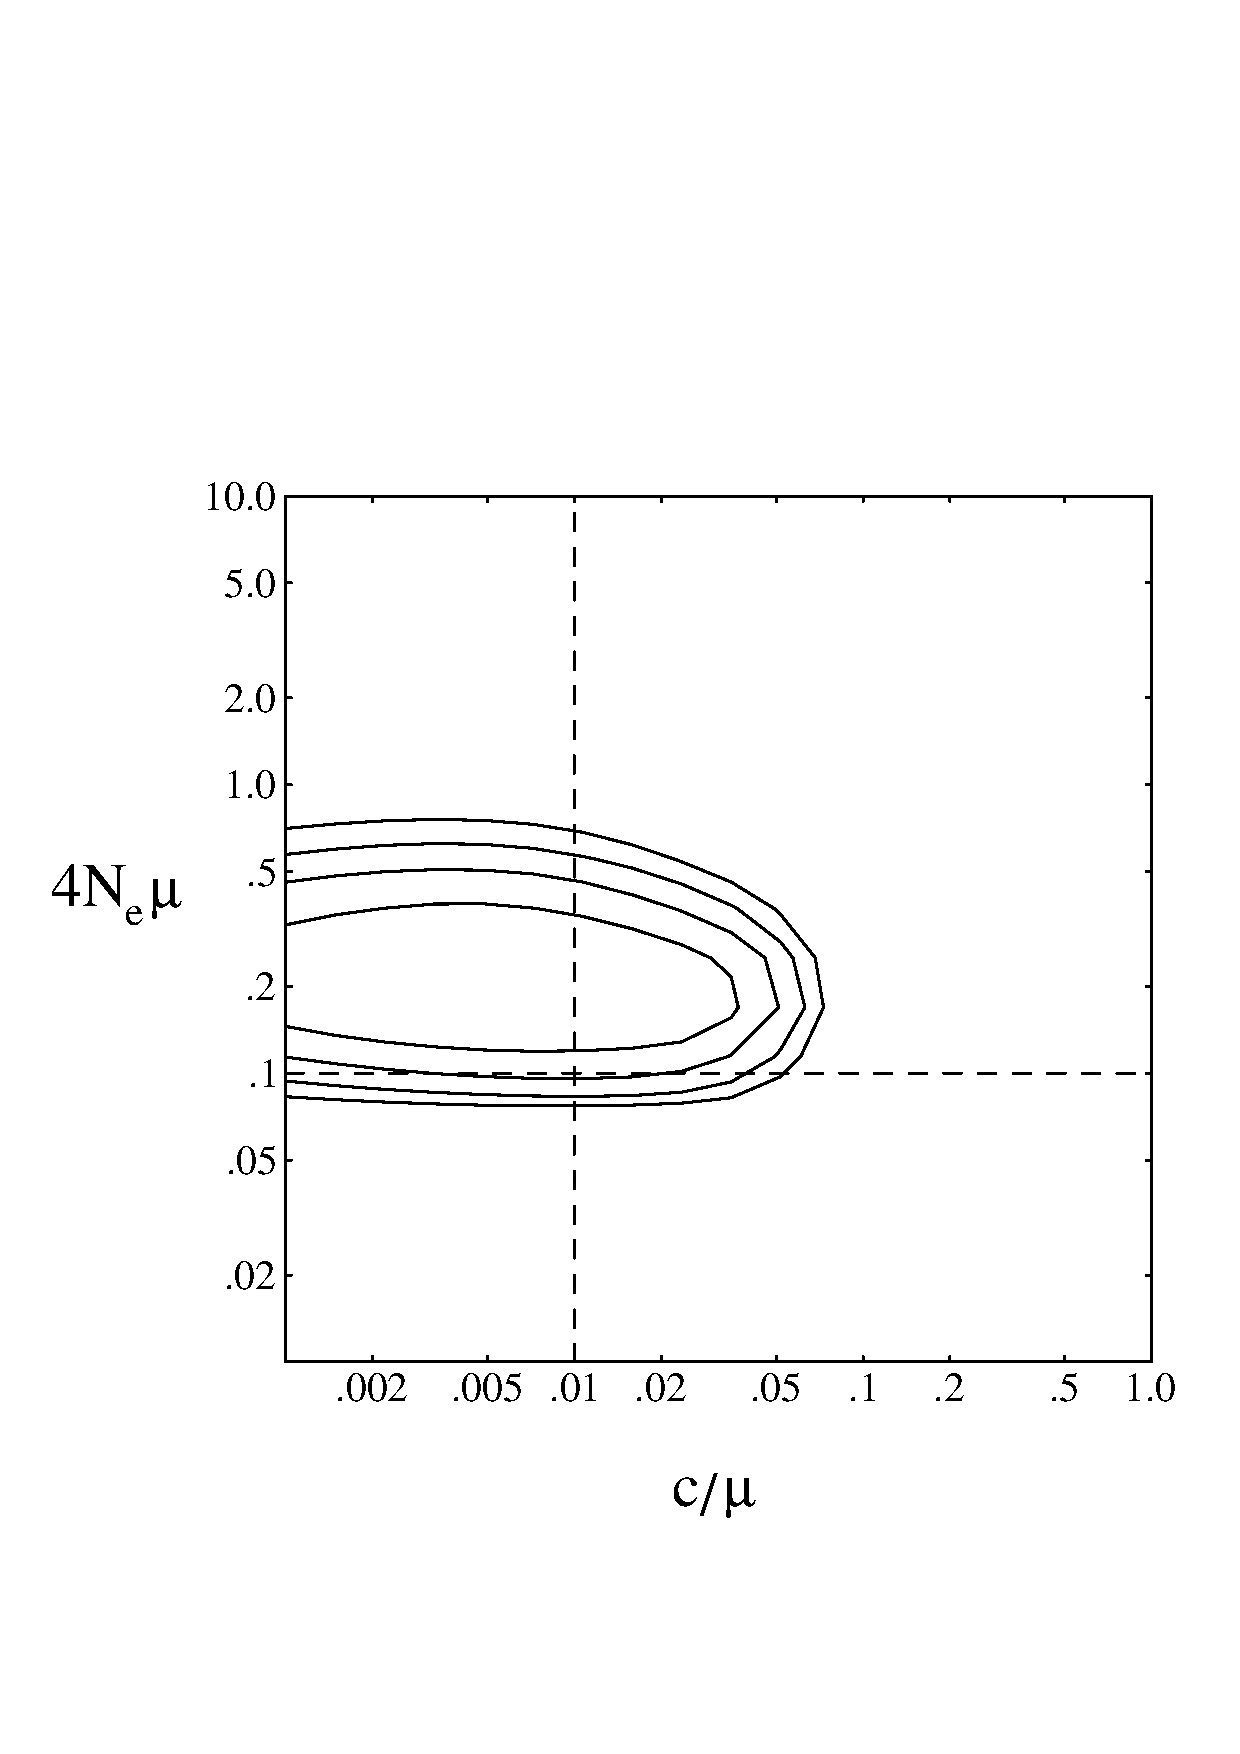
\includegraphics[width=6in]{fig6.idraw}
{\caption ~~}
\end{center}
\end{figure}
\end{document}

